\documentclass[12pt]{article}

\usepackage[a4paper,margin=2cm,top=2cm,bottom=2cm,xetex]{geometry}
\usepackage[utf8]{inputenc}
\usepackage{color,xcolor}
\usepackage{graphicx,algorithm,algorithmic,booktabs,multirow, multicol,float,amsfonts}
\usepackage{enumitem}
\usepackage{amssymb}
\usepackage{amsthm}
\usepackage{amsfonts}
\usepackage{mathtools}
\usepackage{flexisym}
\usepackage{algorithm}
\usepackage{algorithmic}
\usepackage{tabularx}
\usepackage{listings}
\usepackage{xepersian}
\usepackage{amsmath}
\usepackage{physics}


\DeclareFixedFont{\ttb}{T1}{txtt}{bx}{n}{12} % for bold
\DeclareFixedFont{\ttm}{T1}{txtt}{m}{n}{12}  % for normal

% Custom colors
\usepackage{color}
\definecolor{deepblue}{rgb}{0,0,0.5}
\definecolor{deepred}{rgb}{0.6,0,0}
\definecolor{deepgreen}{rgb}{0,0.5,0}

\usepackage{listings}

% Python style for highlighting
\newcommand\pythonstyle{\lstset{
language=Python,
basicstyle=\ttm,
morekeywords={self},              % Add keywords here
keywordstyle=\ttb\color{deepblue},
emph={MyClass,__init__},          % Custom highlighting
emphstyle=\ttb\color{deepred},    % Custom highlighting style
stringstyle=\color{deepgreen},
frame=none,                         % Any extra options here
showstringspaces=false
}}


% Python environment
\lstnewenvironment{python}[1][]
{
\pythonstyle
\lstset{#1}
}
{}

% Python for external files
\newcommand\pythonexternal[2][]{{
\pythonstyle
\lstinputlisting[#1]{#2}}}

% Python for inline
\newcommand\pythoninline[1]{{\pythonstyle\lstinline!#1!}}

%\usepackage{mathtools}

\DeclareFontFamily{U}{matha}{\hyphenchar\font45}
\DeclareFontShape{U}{matha}{m}{n}{ <-6> matha5 <6-7> matha6 <7-8>
matha7 <8-9> matha8 <9-10> matha9 <10-12> matha10 <12-> matha12 }{}
%\DeclareSymbolFont{matha}{U}{matha}{m}{n}
%
%\DeclareMathSymbol{\nvartrianglelefteq}{\mathrel}{matha}{"9E}
%\DeclareMathSymbol{\vartrianglelefteq}{\mathrel}{matha}{"9C}

\newcount\HWcnt
\def\ttmp#1#2#3#4#5#6#7#8#9|{\def\Wjob{#9}}%
\expandafter\ttmp\jobname |
\def\ttmp#1#2#3{\global\HWcnt=#2#3}
\expandafter\ttmp\Wjob

\settextfont[Scale = 1.0 ,
             BoldFont = *Bd ,
             ItalicFont = *It ,
             BoldItalicFont = *BdIt ,
             Extension = .ttf
            ]{XB Niloofar}
\ExplSyntaxOn
\cs_set_eq:NN
\etex_iffontchar:D
\tex_iffontchar:D
\cs_undefine:N \c_one
\int_const:Nn \c_one { 1 }
\ExplSyntaxOff
\setdigitfont[Scale = 1.0 ,
             BoldFont = *Bd ,
             ItalicFont = *It ,
             BoldItalicFont = *BdIt ,
             Extension = .ttf
            ]{XB Niloofar}
\renewcommand{\baselinestretch}{1.2}
\pagestyle{empty}

\makeatletter
\def\abj@num@i#1{%
	\ifcase #1\or الف\or ب\or ج\or د\or ه\or و\or ز\or ح\or ط\fi \ifnum #1=\z@ \abjad@zero \fi
}
\renewcommand{\theenumi}{\abjad{enumi}}
\renewcommand{\labelenumi}{\theenumi)}
\long\def\makeHead#1{%
	\begin{center}\large
		\begin{tabular}{@{}p{.33\linewidth}<{\hfill}@{}>{\hfil}p{.33\textwidth}<{}@{}>{\hfill}p{.33\textwidth}@{}}
            \textbf{تمرین ۱} & & \textbf{ایمان محمدی - 99102207} \\[.5ex]
            \textbf{نیم‌سال دوم ۱۴۰۱-۱۴۰۲} & &  \textbf{ زمان آپلود: #1}\\[.5ex] \hline\hline
		\end{tabular}
	\end{center}\smallskip
%	\def\theenumii{\arabic{enumii}}\def\theenumi{\alph{enumii}}\def\labelenumi{\theenumi)}\def\labelenumii{\theenumii)}%
}

\newcommand{\Rule}{\ \hfill\rule{\linewidth}{0.5pt}\hfill\ \par\vspace*{-2ex}\par}
\newcommand{\DescRule}{\ \hfill\rule{\linewidth}{1pt}\hfill\ \vspace*{-2ex}\par}
\def\rank{\mathop{\mathrm{rank}}\nolimits}

\begin{document}
\makeHead{۲۹ فروردین}
\begin{description}
%	\item{} \noindent
مهلت تحویل این تمرین ۰۸/۰۹/۱۴۰۱ است. شما در مجموع ترم  ۲۰ روز تاخیر مجاز دارید که مدیریت آن با خودتان است. در
ضمن برای هر تمرین شما تا سه روز بعد از ددلاین مجاز به ارسال پاسخ هستید و پس از آن به هیچ عنوان پاسخی از شما پذیرفته
نخواهد شد. پس از ساعات مجاز تاخیر، به ازای هر روز تاخیر،  ٣٠ درصد از نمره شما کسر خواهد شد.
	
%	\DescRule

	\item{\textbf{سوال 1.}} سوال ۱


برای هر کدام از زبان‌های منظم زیر، یک ماشین متناهی قطعی طراحی می‌کنیم که رشته‌های آن زبان را بپذیرد.

\subsection*{۱.۱.۱}

فرض می‌کنیم 
$$N = (Q, \Sigma, \delta, q_0, F)$$
یک DFA با شرایط زیر باشد:
\begin{align*}
	Q &= P(\Sigma)\\
	\Sigma &= \{p,q,r,s\} \\
	\delta(q,a) &= q \cup a \\
	q_0 &= \{\} \\
	F &= \{q \mid |q| \neq 4\}
\end{align*}
درستی این DFA از تعریف آن آشکار است. بدین شکل که آن همه‌ی رشته‌های قابل تعریف روی الفبای مذکور را که هر کدام فاقد دست کم یکی از این کاراکترها هستند، خروجی می‌دهد.

\subsection*{۲.۱.۱}

فرض می‌کنیم 
$$N = (Q, \Sigma, \delta, q_0, F)$$
یک DFA با شرایط زیر باشد:
(در این‌جا $\pi(q)$ مجموعه‌ی همه‌ی جایگشت‌های رشته‌ی $q.$ می‌باشد.)
\begin{align*}
	Q &= \{(?, ?, ?, ?) | ? \in \{a, b, c, .\}\} \\ 
	\Sigma &= \{a,b,c\} \\
	\delta(q, a) &= \begin{cases}
		q & |q| = 4 \land q \notin F  \\
		q \ll a & O.w
	\end{cases} \\ 
	q_0 &= \{., ., ., .\} \\
	F &= \{q \mid q \notin B\} \\
	B &= \{(bbbb), (abba), (cbbc), (acba), (abca), (cabc), (cbac)\} \\ &\cup \pi(bbba) \cup \pi(bbbc)\cup \pi(bbac)
\end{align*}

\subsection*{۲.۱}

از استقرا استفاده می‌کنیم برای اثبات این بخش. در ابتدا پایه‌ی استقرا را تعریف کرده و سپس گام استقرا را اثبات می‌کنیم تا اثبات تکمیل شود. این‌جا روی طول
$\omega$
استقرا می‌زنیم.
پایه‌ی استقرا: فرض می‌کنیم طول $\omega$ صفر است. در نتیجه با توجه به تعریف، داریم:
\begin{align*}
	\hat{\delta}^{*}(q_0, \epsilon) &= \{q_0\} \\
	\delta^{*}(\{q_0\}, \epsilon) &= \{q_0\} \\
	\implies \hat{\delta}^{*}(q_0, \epsilon) &= \delta^{*}(\{q_0\}, \epsilon)
\end{align*}
حالا فرض می‌کنیم برای $\omega = \omega_1\omega_2\dots\omega_k$ نیز درست باشد. پس داریم:
\begin{align*}
	\hat{\delta}^{*}(q_0, \omega_1\dots\omega_k) &= \delta^{*}(\{q_0\}, \omega_1\dots\omega_k) \\
	\hat{\delta}^{*}(q_0, \omega_1\dots\omega_{k+1}) &= \hat{\delta}(\hat{\delta}^{*}(q_0, \omega_1 \dots \omega_{k}), w_{k + 1}) = \bigcup_{r \in \hat{\delta}^{*}(q_0, \omega_1 \dots \omega_{k})} \hat{\delta}(r, w_{k + 1})
	\\ \delta^{*}(\{q_0\}, \omega_{1}\dots\omega_{k + 1}) &= \delta(\delta^{*}(\{q_0\}, \omega_1 \dots \omega_{k}), \omega_{k+1}) = \bigcup_{r \in \delta^{*}(\{q_0\}, \omega_1 \dots \omega_{k}))} \hat{\delta}(r, w_{k + 1}) \\
	\implies \hat{\delta}^{*}(q_0, \omega_1\dots\omega_{k + 1}) &= \delta^{*}(\{q_0\}, \omega_1\dots \omega_{k+1}) \blacksquare
\end{align*}
در نتیجه اثبات کامل است.

\subsection*{۳.۱}

در این بخش کافی‌ست برای هر یک از موارد گفته شده، یک مثال نقض آوریم. یک ماشین ساده‌ی دو استیتی را نیز اگر در نظر بگیریم می‌توانیم رد کنیم موضوع مطرح شده را.

در مثال زیر، ماشین M به صورت 
$$M = (Q, \Sigma, \delta, q_0, F)$$
می‌باشد.
\\
\\
\begin{center}
	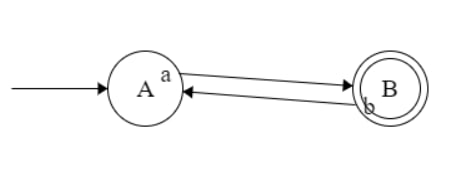
\includegraphics{DFA1}
	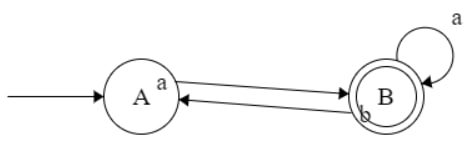
\includegraphics{DFA2}
\end{center}
در ماشین بالا ابتدا رشته‌های به فرمت
$a\{ba\}*$
را می‌پذیریم. اگر از یکی دو روش گفته شده استفاده کنیم، ماشین پایینی بدست می‌آید. این ماشین رشته‌های به فرمت
$a\{ba\}*a*$
را می‌پذیرد، همچنین رشته‌های اشتباهی نیز می‌پذیرد مانند $aaaaba$؛ پس این روش‌ها حتما درست کار نمی‌کنند و مثال نقض زدیم.

برای حالت بعدی نیز داریم که ماشین N به صورت 
$$N = (Q, \Sigma, \delta, q_0, F)$$
می‌باشد.
در این ماشین، رشته‌های به فرمت $b\{ab\}*$ پذیرفته می‌شوند. حالا اگر به روش گفته شده در شرح سوال، یال اضافه کنیم، رشته‌های به فرمت 
$a*b\{ab\}*$
را هم می‌پذیریم، اما برای مثال رشته‌ای مانند $baaaab$ را هم می‌پذیریم که مثال نقض است و در نتیجه روش گفته شده لزوما درست کار نمی‌کند.
\\
\\
\begin{center}
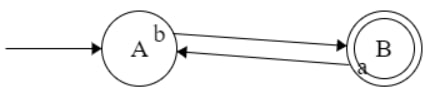
\includegraphics{DFA4}
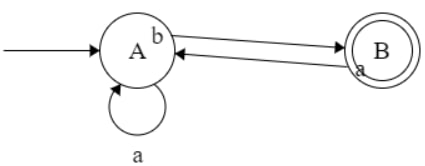
\includegraphics{DFA3}
\end{center}


	
	\Rule
	
	\item{\textbf{سوال 2.}} \section*{1.2}

\subsection*{الف}
برای اثبات بستگی زبان‌های مستقل از متن دربرابر عمل الحاق، دو گرامر زیر را در نظر می‌گیریم:
\[
G_1 = (V_1, \Sigma_1, R_1, S_1) \quad G_2 = (V_2, \Sigma_2, R_2, S_2)
\]
گرامر الحاق این دو به شکل زیر خواهد بود:
\[
G_T = (V_1 \cup V_2 \cup \{S_0\}, \Sigma_1 \cup \Sigma_2, R_1 \cup R_2 \cup \{S_0 \to S_1 S_2\}, S_0)
\]
که در آن یک نشان‌دهندهٔ جدید، یعنی $S_0$، تعریف شده است و یک ارتباط جدید، $S_0 \to S_1 S_2$، برقرار شده است. این گرامر نشان‌دهندهٔ عمل الحاق است، بنابراین زبان‌های مستقل از متن دربرابر این عمل بسته هستند.

\subsection*{ب}
حالا یک گرامر دلخواه، $G_1 = (V_1, \Sigma_1, R_1, S_1)$، را در نظر بگیرید. برای عملگر $*$، گرامری را می‌توان به شکل زیر در نظر گرفت:
\[
G_{*} = (V_1 \cup \{S_{*}\}, \Sigma_1, R_1 \cup \{S_{*} \to S_1 S_{*} \,|\,\epsilon\}, S_{*})
\]
مانند بخش الف، یک نشان‌دهندهٔ جدید، $S_{*}$، در نظر گرفته شده است و با افزودن قاعده $S_{*} \to S_1 S_{*} \,|\,\epsilon$ به مجموعه قواعد، می‌توان عملگر $*$ را پیاده ساخت. پس زبان‌های مستقل از متن نسبت به این عملگر نیز بسته خواهند بود.

\section*{2.2}

\subsection*{الف}
با توجه به زبان مستقل از متن ارائه شده، زبان زیر را در نظر بگیرید:
\[
L = \{a^m b^k c^n \,|\, m,n \geq 0 \,and\, (m = k + n \,or\, k = m + n \,or\, n = k + m)\}    
\]
با توجه به بستگی زبان‌های مستقل از متن دربرابر عمل اجتماع، می‌توان زبان بالا را به سه زبان مجزا تقسیم کرد و با اثبات مستقل بودن هر یک از آن‌ها، در نهایت به مستقل بودن زبان $L$ می‌رسیم. بنابراین، زبان‌های زیر را در نظر بگیرید:
\begin{align*}
	L_1 &= \{a^m b^k c^n \,|\, m = k + n\} \\
	L_2 &= \{a^m b^k c^n \,|\, n = k + m\} \\
	L_3 &= \{a^m b^k c^n \,|\, k = m + n\}
\end{align*}
در ابتدا برای زبان $L_1$، گرامر مستقل از متن زیر را می‌نویسیم:
\begin{align*}
	S &\to a S c \,|\, X \\
	X &\to a X b \,|\, \epsilon
\end{align*}
که در آن جمع تعداد تکرار حروف $c$ و $b$ با $a$ برابر خواهد بود، چرا که برای هر $a$، یک $c$ یا یک $b$ وجود دارد. بنابراین، گرامر زبان $L_1$ مستقل از متن است.

به همین ترتیب، برای زبان $L_2$، گرامر مستقل از متن زیر را در نظر بگیرید:
\begin{align*}
	S &\to a S c \,|\, X \\
	X &\to b X c \,|\, \epsilon
\end{align*}
که در آن جمع تعداد تکرار $a$ و $b$ برابر با $c$ خواهد بود. بنابراین، این زبان نیز یک زبان مستقل از متن است.

در نهایت، برای زبان $L_3$، می‌توان دو زبان مستقل از متن زیر را الحاق کرد:
\[
L_4 = (a^m b^k \,|\, m = k) \quad
L_5 = (b^k c^n \,|\, k = n)     
\]
که می‌دانیم این دو زبان مستقل از متن هستند، پس الحاق آنها نیز مستقل از متن بوده و در نیتجه زبان $L$ مستقل از متن خواهد بود.

برای بخش بعدی، زبان زیر را در نظر بگیرید:
\[
L = \{a^{m_1} b^{k_1} c^{n_1} \dots a^{m_i} b^{k_i} c^{n_i} \,|\, i \geq 0 \,and\, \forall j \leq i \, m_j, n_j \geq 0 \,and\, k_j = 3m_j + 4n_j\}    
\]
از آنجایی که زبان‌های مستقل از متن نسبت به عمل $*$ بسته هستند، می‌توان زبان $L$ را به این صورت تقلیل داد:
\[
L = (L_1)^{*} \implies L_1 = (a^m b^k c^n \,|\, k = 3m + 4n)    
\]
بنابراین کافی است نشان دهیم زبان $L_1$ مستقل از متن است. برای اینکار، دو زبان زیر را با گرامر متناظر با آنها در نظر می‌گیریم:
\[
L_2 = (a^m b^k \,|\, k = 3m) \quad S \to aSbbb \,|\, \epsilon    
\]
\[
L_3= (b^k c^n \,|\, k = 4n) \quad S \to bbbbSc \,|\, \epsilon    
\]
با الحاق این دو زبان، $L_1$ ساخته می‌شود. از آنجایی که هرکدام از آنها مستقل از متن هستند و عملگر الحاق نیز نسبت به این کار بسته است، در نهایت زبان $L$ یک زبان مستقل از متن خواهد بود.

	
	\Rule
	
	\item{\textbf{سوال 3.}} \subsection*{۱.۳}

زبان
$L_1$
یک زبان منظم می‌باشد چون می‌توانیم برای آن یک 
dfa
به صورت زیر طراحی کنیم.

\begin{center}
	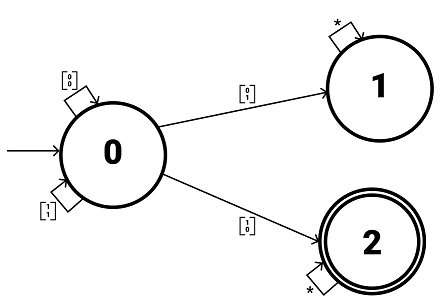
\includegraphics{DFA24}
\end{center}

به ازای دریافت حالت
$\binom{1}{0}$
می‌دانیم عدد بالایی بزرگتر خواهد بود و برای
$\binom{0}{1}$
عدد پایینی. در مابقی حالات در وضعیت خود می‌مانیم.

برای زبان
$L_2$
می‌دانیم هر رشته‌ای که در بالا تکرار شود معکوس همان رشته می‌بایست در پایین تکرار شود. بنابراین یک حالت آن می‌تواند به صورت زیر باشد.
$$\mqty[1^p & 0^p \\ 0^p & 1^p] = x y z$$
که در آن
$|x y| \leq p$
و
$|y| > 0$
خواهند بود. پس می‌توان گفت
$y$
به صورت
$\binom{1^k}{0^k},\, 0 < k < p$
خواهد بود.

حالا در رشته‌ی می‌بینیم
$x y^2 z$
که به
$\mqty[1^{p + k} & 0^{p + k} \\ 0^p & 1^p]$
برمی‌خوریم، بنابراین این زبان را نمی‌توان با
DFA
خاصی توصیف کرد و یک زبان نامنظم است.

\subsection*{۲.۳}

با استفاده از لم پمپاژ اثبات می‌کنیم که این زبان منظم نیست. طبق لم پمپاژ عدد p را پیدا می‌کنیم در ابتدا.

یک رشته‌ی شامل p تا پرانتز باز و p تا پرانتز بسته در نظر بگیرید.

با توجه به این‌که

$$s = xyz,\,|x y| < p, |y| > 0$$

پس داریم که y شامل تعدادی پرانتز باز است فقط.

حالا با توجه به لم پمپاژ به ازای هر i، یک عضو زبان گفته می‌شود به هر 
$x y^i z$

اما در این‌جا با قرار دادن i به مقدار ۲، تعداد پرانتزهای باز از بسته بیشتر می‌شود و رشته خوش‌پرانتز نیست. 

در نتیجه لم پمپاژ صدق نمی‌کند و زبان منظم نیست.

\subsection*{۳.۳}

می‌توان با استفاده از زبان
$L_1 = \{a^i b^i\,|\,i > 0\}$
نشان داد که زبان
$L_2$
نامنظم است. برای زبان
$L_2$
زبانی را تعریف می‌کنیم که اشتراکش با آن برابر زبان
$L_1$
شود. برای تعریف چنین زبانی می‌توانیم یک زبان که با ۱ شروع می‌شود تعریف کنیم به طوری که حتما ۱ یا ۰ داشته باشد و به تعداد دلخواه تکرار شود، یعنی داریم.
$$L_4 = \{11^{*} 00^{*}\} \implies L_2 \cap L_4 = L_1$$
می‌دانیم که زبان
$L_4$
منظم است چون می‌توان یک
DFA
برای آن طراحی کرد که از دارای سه استیت بوده و با ورود ۱ از استیت شروع به استیت شماره یک می‌رود. در استیت شماره یک با دریافت ورودی صفر به استیت شماره دو و با گرفتن ورودی یک در خود بماند. برای استیت شماره دو هم فقط در حالتی که ورودی، صفر باشد، در خود می‌ماند و حالت
$accept$
خواهد بود.
حالا چون اشتراک زبان
$L_2$
با زبان دیگری منظم نبود، پس این زبان نامنظم است.

برای بخش دوم این سوال، فرض می‌کنیم 
$L_5$
زبانی شامل تمام رشته‌های شامل دقیقا یک عدد ۰ است. این زبان منظم است و عبارت منظم آن به شکل 
$$
(1 \cup 2)^* 0(1 \cup 2)^*
$$
است.
حالا اگر 
$L_3$
منظم باشد، با توجه به خواص بستاری زبان 
$L_3 \cap L'$
هم منظم است که این زبان معادل زبان
$\{ 01^y2^y | y \geq 0 \}$

حال چون یک DFA برای این زبان وجود دارد که 
$0 \notin \{ 1, 2\}$
پس 	
quotient left
این زبان نسبت به 
$\{ 0 \}$
می‌شود:
$\{ 1^y2^y | y \geq 0 \}$
که زبان نامنظمی است و تناقض داریم و بدست می‌آید که 
$L_3$
نامنظم است.
	
	\Rule
	
	\vspace*{+10ex}\ \hfill\textbf{موفق باشید.}
\end{description}
\end{document}